\section{Nelson/Siegel and Svensson method}
\label{sec:nels-svenss-meth}


\includegraphics[width=0.3in]{baustelle} longer introduction

\cite{Nelson1987} propose a parsimonious  model of  the instantaneous forward rate as a solution to a second-order differential equation for the case of equal roots.

\begin{equation}
  \label{eq:laguerre}
  f(m,\bm{b}) = \beta_0+\beta_1\exp\left(-\frac{m}{\tau_1}\right)+\beta_2\left[\left(\frac{m}{\tau_1}\right)\exp\left(-\frac{m}{\tau_1}\right)\right]
\end{equation}


The spot rate is the average of the instantaneous forward rates. 

\begin{equation}
  \label{eq:intspotrate}
  s(m,\bm{b})=\frac{1}{m}\int_0^mf(m,\bm{b})\,dm
\end{equation}


\begin{equation}
  \label{eq:nelson-spot}
   s(m,\bm{b}) = \beta_0 + \beta_1\frac{1-\exp(-\frac{m}{\tau_1})}{\frac{m}{\tau_1}} + \beta_2\left(\frac{1-\exp(-\frac{m}{\tau_1})}{\frac{m}{\tau_1}} - \exp(-\frac{m}{\tau_1})\right)
\end{equation}



\begin{figure}[htb]
  \label{fig:curveshape}
  \caption{Model curves}
\begin{center}
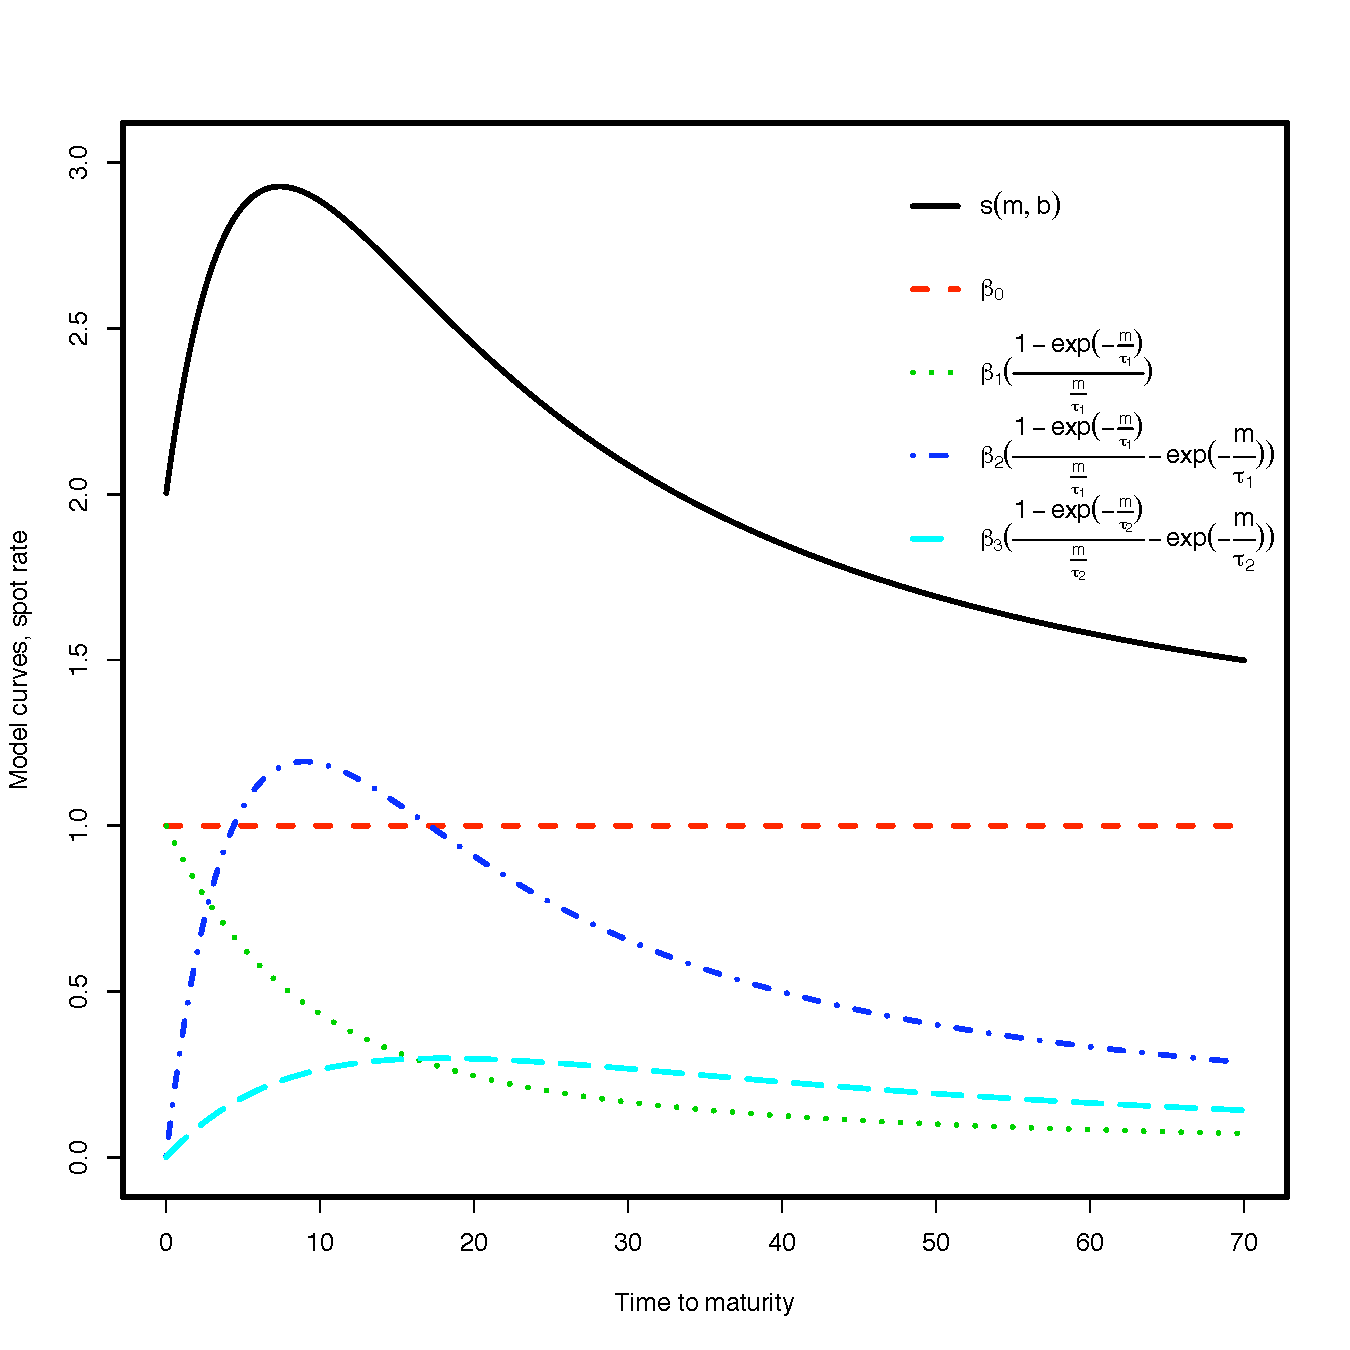
\includegraphics[width=0.7\textwidth]{curveshape}
\end{center}
\end{figure}


%\input{curveshape.tex}
 
\cite{Svensson1994} extension


\begin{multline}\label{eq:svensson-spot}
    s(m,\bm{b}) = \beta_0 + \beta_1\frac{1-\exp(-\frac{m}{\tau_1})}{\frac{m}{\tau_1}} + \beta_2\left(\frac{1-\exp(-\frac{m}{\tau_1})}{\frac{m}{\tau_1}} - \exp(-\frac{m}{\tau_1})\right) \\+ \beta_3\left(\frac{1-\exp(-\frac{m}{\tau_2})}{\frac{m}{\tau_2}} - \exp(-\frac{m}{\tau_2})\right)
\end{multline}



with a parameter vector ${\bm{b}} = \left(\beta_0,\beta_1,\beta_2,\tau_1,\beta_3,\tau_2\right)$.

Figure \ref{fig:curveshape} shows the impact of the different terms in the spot rate function. The parameters have the following interpretations: \ref{fig:curveshape}

\begin{itemize}
\item $\beta_0$ is the asymptotic value of the spot rate function $\lim_{m\to\infty}s(m,\bm{b})$, which can be seen as long-term interest rate.
\item $\beta_1$ determines the rate of convergence which with the spot rate function approaches its long-term trend, and $\beta_0+\beta_1$ is the starting value of the curve at the short end. The slope will be negative if $\beta_1>0$ and vice versa.
\item $\beta_2$ determines the size and the form of the hump. $\beta_2 >0$  results in a hump at  $\tau_1$, whereas $\beta_2<0$ produces a U-shape.
\item $\tau_1>0$ specifies the location of the first hump or the U-shape on the curve
\item $\beta_3$, analogously to $\beta_2$, determines the size and form of the second hump.
\item $\tau_2>0$ specifies the position of the second hump.
\end{itemize}

The discount factor for any maturity can be calculated as follows. 

\begin{displaymath}
d(m_{ij})=e^{-m_{ij}s(m_{ij},b)},
\end{displaymath}

where $s(m_{ij},b)$ is the Nelson/Siegel or Svensson spot rate function defined in \eqref{eq:nelson-spot} and \eqref{eq:svensson-spot}.

We optimize the objective function in \eqref{eq:optimalparam}. The above specification of the discount function leads to nonlinear optimization. Good starting values for the parameter vector are important to find a global minimum. Instead of the pricing errors, it is common to minimize the yield errors. Calculating the yield-to-maturities of the theoretical bond prices is easy to solve numerically, because \eqref{eq:yield} has only one real root. The difference to the minimization of the pricing errors is $\dots$.

When minimizing the unweighted price errors, bonds with a longer maturity get a higher weighting, because they are more sensitive to changes in prices, which leads to a less accurate fit at the short end. Solutions to this heteroskedasticity problem are to use weights for the price errors, or to minimize the yield errors. A possible specification for the weights is based on the inverse of the duration as in \eqref{eq:durationweight}.


\includegraphics[width=0.3in]{baustelle} describe heteroskedasticity problem of estimation with unweighted price errors

%%% Local Variables: 
%%% mode: latex
%%% TeX-master: "jss-termstrc"
%%% End: 
